
\section{Implementation of Classifiers}
%This section describes the custom implementation of the \textit{Decision Tree} and \textit{Neural Network} classification methods. Each method's \textit{Python} implementation is first thoroughly described and then its correctness is being proved.


\subsection{Decision Tree}
\subsubsection{Details on Implementation}

The decision tree classifier was implemented using three different classes:


\begin{enumerate}
    \item \class{Node()} - Low level data-structure used to represent nodes in a decision tree
    
    \item \class{DecisionTree()} - Decision tree parent class which implements the building process of a tree (fitting) 
    
    \item \class{DecisionTreeClassifier()} - Client-facing constructor for setting up the model
\end{enumerate}
\vspace{10pt}

% Node Class
The \class{Node()} class is a data structure holding information about a single split at any level in a decision tree. There are three types of \code{Node} objects. 
A node can be of type (\code{self.type}) \code{root}, \code{internal} or \code{leaf}. Root and internal nodes are constituted in the same way. They hold the indices of the subset of the original training data that are considered for splitting at the node (\code{self.values}) and information about which feature index (\code{self.p}) provides the best cut point $s$ (\code{self.val}) to partition the subset into two nodes. These two nodes are then pointed to in the \code{self.left} and \code{self.right} attributes. Using this linked structure, the decision tree can be traversed until a leaf node is reached for classifying data points.
Leaf nodes do not contain any pointers to other nodes and thus also do not define a best-split. Instead, they save information about the decision being made in that leaf (decision region), which is saved in the \code{self.predict_proba} and \code{self.predict} attributes. 
\newline

% Decision Tree Class
The \class{DecisionTree()} is the core class as it implements the construction (fitting) of the decision tree as well as prediction of classes for the given data. A call to \code{.fit()} with a feature matrix $X$ and a target vector $y$ representing categorical classes initialises the root (\code{self.root}) to a \code{Node} instance with all indices in the training data and then recursively splits the node until full purity or a stop-criterion is reached. The recursive call to \code{.split()} first finds the best possible split through the private, helper function \code{._best_split()} for the data in the node to be split. The function returns the index of the feature and the corresponding value for which the weighted loss (impurity measure) was minimal, alongside the weighted loss itself. All are stored in the current node to be split.
Finally, the indices of the data points in the left and right child (found from the best split) are computed and initialised as \class{Node} objects. If the resulting child is pure (ie. only contains data points of the same class) or a stopping criterion is reached, the recursion ends and the node is turned into a \code{leaf} node. Otherwise, the \code{.split()} function is recursively called on the children of the former node. On a call to \code{.predict()}, the fitted tree is traversed until a leaf node is reached. The decision tree predicts to the majority class in the leaf node (\code{self.predict} attribute of leaf).

% Decision Tree Classifier
%The \class{DecisionTreeClassifier()} is the class to be used by clients. % it implements evaluate leaf 


\subsubsection{Correctness}
In theory, a decision tree classifier is able to overfit any unique training data to 100\% training accuracy. It was therefore tested, whether the custom implementation has this property. Figure \ref{assert_dt_overfit} shows the training and test accuracy on a random 70-30 split of the \textit{Iris Dataset} with deleted duplicate data points for the custom \class{DecisionTreeClassifier()} trained on the first two features in the data and stopped at increasing depths (from 1 to 20). As expected, the training accuracy continuously increases, since for each added depth of training the purity of the leaves increases. A decision tree with maximum depth of 11 is enough to entirely overfit the data and result in 100\% training accuracy. Overall, the implementation behaves exactly as expected. 
\newline

\begin{figure}[ht]
\centering
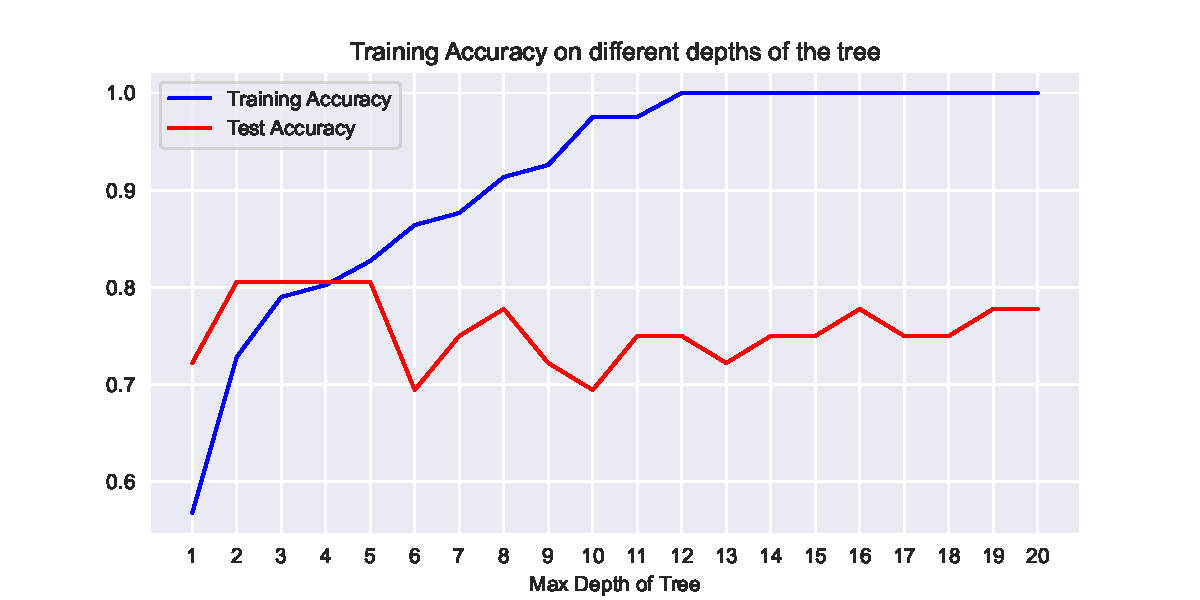
\includegraphics[scale=0.6]{figures/assert_dt_overfit.pdf}
\captionsetup{justification=centering,margin=2cm}
\caption{Training and Test Accuracy on Iris Data (Feature 1 and 2) for increasing \textit{Max Depth} Hyperparameter}
\label{assert_dt_overfit}
\end{figure}

Figure \ref{assert_dt_toydata} depicts the 2d-decision regions constructed for decision trees trained to different maximum depths on the \textit{Iris} and \textit{Circles Data sets} in row $1$ and $2$ respectively. The left-most plots show the decision regions for a tree trained to depth $1$. This means, only a single split is allowed. With larger maximum depths, the models learn more and more of the variation (and noise) in the training data and finally overfit the training data to 100\% training accuracy. Again, the decision regions constructed are sensible and conform with a reference implementation of \textit{sci-kit learn}.
\newline

\begin{figure}[ht!]
\centering
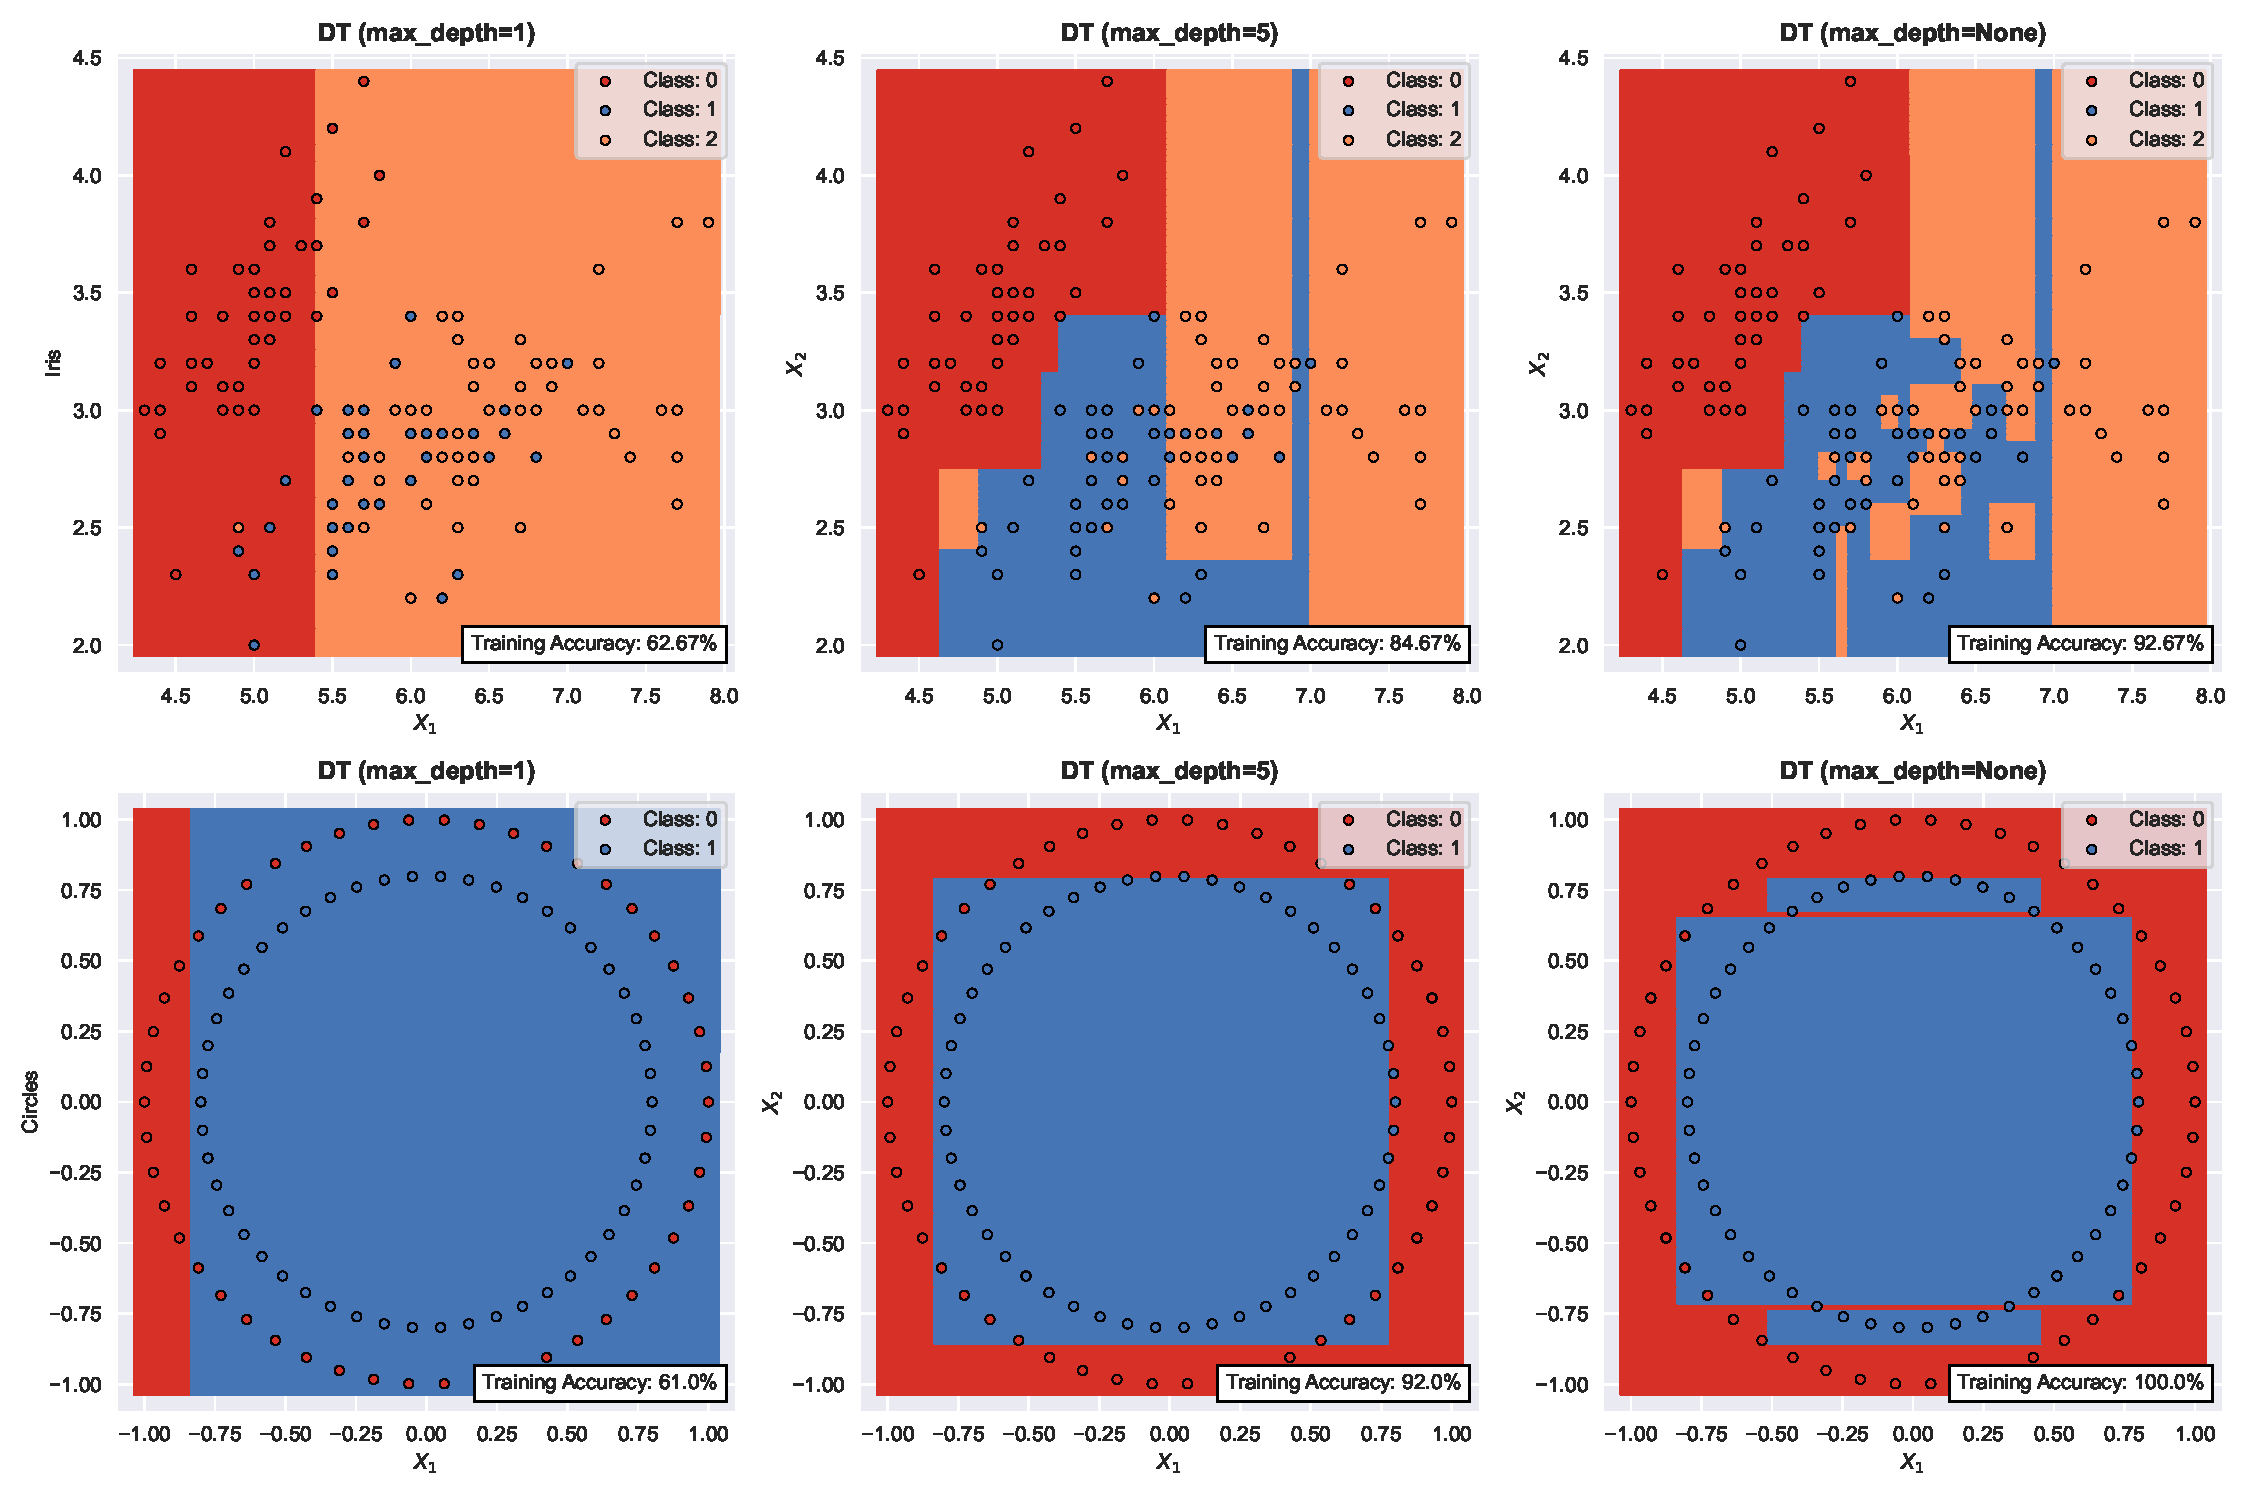
\includegraphics[scale=0.35]{figures/assert_dt_toydata.pdf}
\captionsetup{justification=centering,margin=2cm}
\caption{Performance of Decision Tree on Iris (Row 1) and Circles (Row 2)}
\label{assert_dt_toydata}
\end{figure}
\newpage


% ---------- NEURAL NET
\subsection{Neural Network}
\subsubsection{Details on Implementation}

The \class{NeuralNetworkClassifier()} was implemented using three different classes:

\begin{enumerate}
    \item \class{Var()} - Low-level numeric data type with auto-differentiation  (adapted from \textit{Nanograd} \cite{Autograd})
    \item \class{DenseLayer()} - Fully-connected layer within neural network 
    \item \class{NeuralNetworkClassifier()} - Client-facing class for constructing, training and predicting from neural network
\end{enumerate}
\vspace{10pt}

The \class{Var()} class is low-level numeric data type. It allows for basic numeric operations (such as addition and multiplication) and auto-differentiation. This means, that through storing information about how a \code{Var} instance was created via its parents attribute (\code{self.parents}), the gradient of any \code{Var} instance can be computed.

\begin{comment}
Listing $1$ shows this on a simple example.

% Simple example
\begin{lstlisting}[language=Python, caption=Simple example of Var class functionality]
import Var
a = Var(2)
b = Var(3)
c = a*b
\end{lstlisting}
The variable $c$ will have a \textit{value} $6$ (\code{self.value}) and its \textit{parents} (\code{self.parents}) will be $a$ and $b$. In addition, within the \textit{parents} attribute, it is also noted for each parent, what is the partial derivative of $c$ with respect to it. 
\end{comment}

\begin{figure}[ht]
\centering
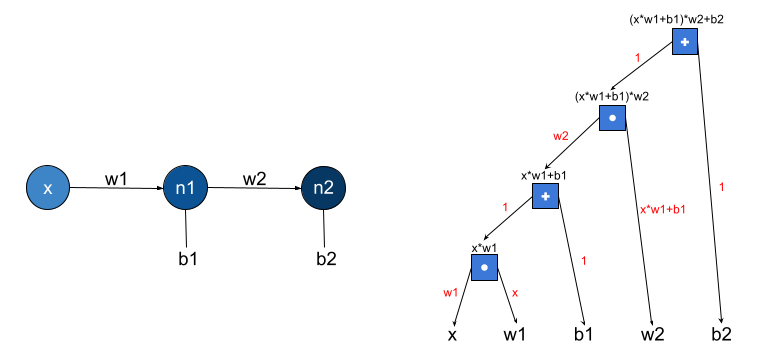
\includegraphics[scale=0.6]{figures/backprop.png}
\captionsetup{justification=centering,margin=2cm}
\caption{A simple network with one feature and one hidden layer (no activation functions) along with a computational dependency tree}
\label{backprop}
\end{figure}

Figure \ref{backprop} demonstrates the \code{Var}'s utility of a forward pass through a highly simplified neural network, where the output $n_2$ is computed through forward passing x as $n_2 = (xw_1+b_1)w_2+b_2$. The right side of the figure shows a dependency tree of this computation, where each node is \code{Var} instance. Red values denote the partial derivative of a given child with respect to its parent. Finally, to compute partial derivatives of any node with respect to any of its descendants, the tree is traversed reversely from the node to the descendant and the product of edge weights is the final partial derivative.

\begin{comment}
the following pseudo algorithm is used:
\begin{enumerate}
    \item Find all paths from the given child to the given descendant
    \item For each path, multiply the edge weights on that path together
    \item Sum over all results of multiplied path weights of step 2.
\end{enumerate}
\end{comment}

This algorithm is a translation of the chain rule. For instance, the partial derivative of $n_2$ with respect to $w_1$ is computed from the \code{Var} tree as:

$$\frac{\partial n_2}{\partial w_1} = 1\cdot w_2 \cdot 1 \cdot x$$


The \class{Var()} then implements a method \code{self.backward()}, which traverses the dependency tree by computing the partial derivative for each node. The partial derivatives are then assigned to the attribute \code{self.gradient} in the respective nodes.
\newline

The \class{DenseLayer()} class serves as a building block for the \class{NeuralNetworkClassifier()}. The class is being initialised with an input and output dimension, as well as an activation function. On initialisation, a weight matrix (\code{self.weights}) is built  based on the provided number of input and output dimensions along with a vector of biases (\code{self.biases}). The weights and biases are initialized from a uniform distribution $[0,1)$ and each element is converted into a \code{Var} instance for the back-propagation to work. The core functionality of the \class{DenseLayer()} class is to feed forward a set of data points through the layer. The \code{self.forward} method takes a matrix \textit{X} of \code{Var} instances. This matrix corresponds either to the output of the previous layer within \class{NeuralNetwork()} or to the feature matrix if the dense layer is the first layer. Finally, it computes the forward pass (using \code{self.weights}, \code{self.biases} and \code{self.activation}) and returns a matrix of \code{Var} instances - the activation of neurons in that layer. The operation is vectorised for performance reasons.
\newline

The \class{NeuralNetworkClassifier()} serves as a wrapper which puts together the preceding two classes and is used to fit the parameters (weights and biases) of each layer. The class is initialised by inputting a list of layers (\code{self.layers}), which are all instances of the  \class{DenseLayer()} class, and the type of a loss function to be used for training the model (\code{self.loss}). To train the network, the method \code{self.fit()} with a feature matrix \textit{X} and target vector \textit{y} needs to be called. In addition, it is possible to specify training hyper-parameters including the \textit{number of batches}, the \textit{number of epochs} and the \textit{learning rate}.  In the training loop, for each epoch all batches are fed forward through the network and their respective losses are propagated back to update the weights in the network. 
Once the neural network is fitted, the \code{self.predict()} method can be used to feed forward data points and get the corresponding predictions from the neural network.

\begin{comment}
\begin{lstlisting}[language=Python, caption=Simple example of Var class functionality]
def forward(self, X):
    return self.activation(X @ self.weights + self.bias)
\end{lstlisting}
\end{comment}

\begin{comment}
In the training loop a randomly selected batch is sent through the network using the \code{self.forward()} method which iterates over all layers and calls their own \code{self.forward()} method. The result of this process is a matrix with $n$ rows and $p$ columns where $n$ is equal to the length of inputted batch and $p$ to the number of output neurons in the last layer. Based on this matrix, loss is computed using \code{self.loss()}. The computed loss is then used to update network's parameters as follows:

\begin{enumerate}
    \item Iterate over all parameters and set their \code{self.gradient} to zero (to avoid accumulation from previous training)
    \item On the computed loss, call \code{self.backward()} in order to compute new gradients of the network's parameters
    \item Again, iterate over all parameters and update their values using their gradient and a given learning rate
\end{enumerate}
\end{comment}


\subsubsection{Correctness}
%The correctness of a neural network implementation is slightly more difficult to show, since it is a black-box model, meaning that its learning process can not be fully comprehended. Nonetheless, we expect some characteristic training behavior for certain settings of neural networks and can, just like for the decision tree, visually inspect the learned decision regions for toy data sets. 

The Universal Approximation Theorem \cite{universal_aprox_theorem} states that a neural network with a single hidden layer is able to approximate any continuous function. Figure \ref{assert_nn_overfit} shows the loss and training accuracy history of the custom neural network implementation trained for 100 training epochs on the Iris Dataset (duplicate data points were removed). The neural network used contained a single hidden, ReLu activated layer of 20 neurons and trained for ten batches per epoch with a learning rate of 0.01. The visualisation of the training history confirms the model's implementation. Due to batch learning, the loss history is slightly choppy, nonetheless the loss is continuously decreasing and maximising the training accuracy to 99\% training accuracy. Overall, the implementation behaves as expected. 

\begin{figure}[ht!]
\centering
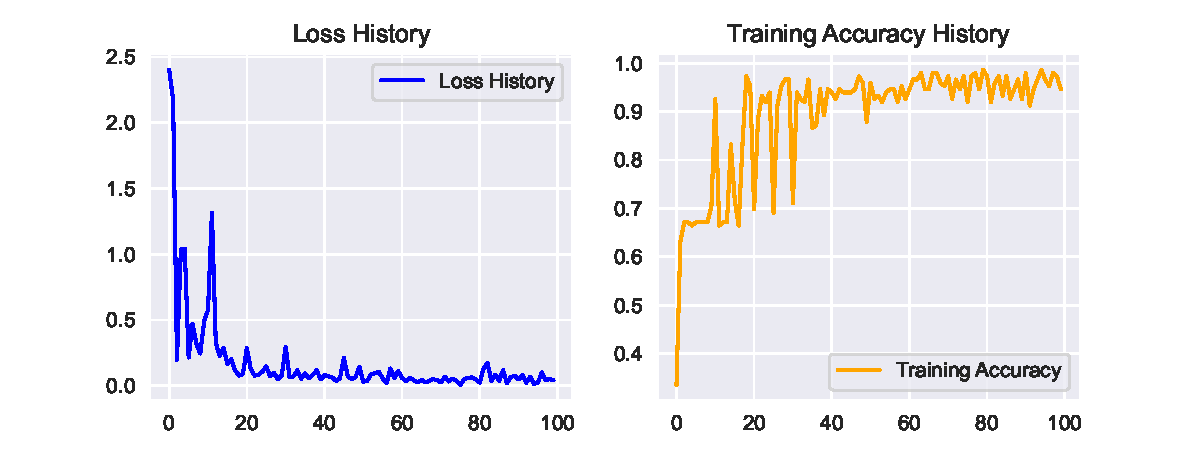
\includegraphics[scale=0.8]{figures/assert_nn_overfit.pdf}
\captionsetup{justification=centering,margin=2cm}
\caption{Overfitting Iris Dataset with Custom Neural Network Implementation}
\label{assert_nn_overfit}
\end{figure}

Figure \ref{assert_nn_toydata} depicts the 2d-decision regions constructed for simple neural networks trained for different amounts of epochs on the \textit{Iris} and \textit{Circles Data sets} in row $1$ and $2$ respectively. The same network architecture was used for both data sets. It is evident, that the neural network is able to learn patterns from the training data.

\begin{figure}[ht!]
\centering
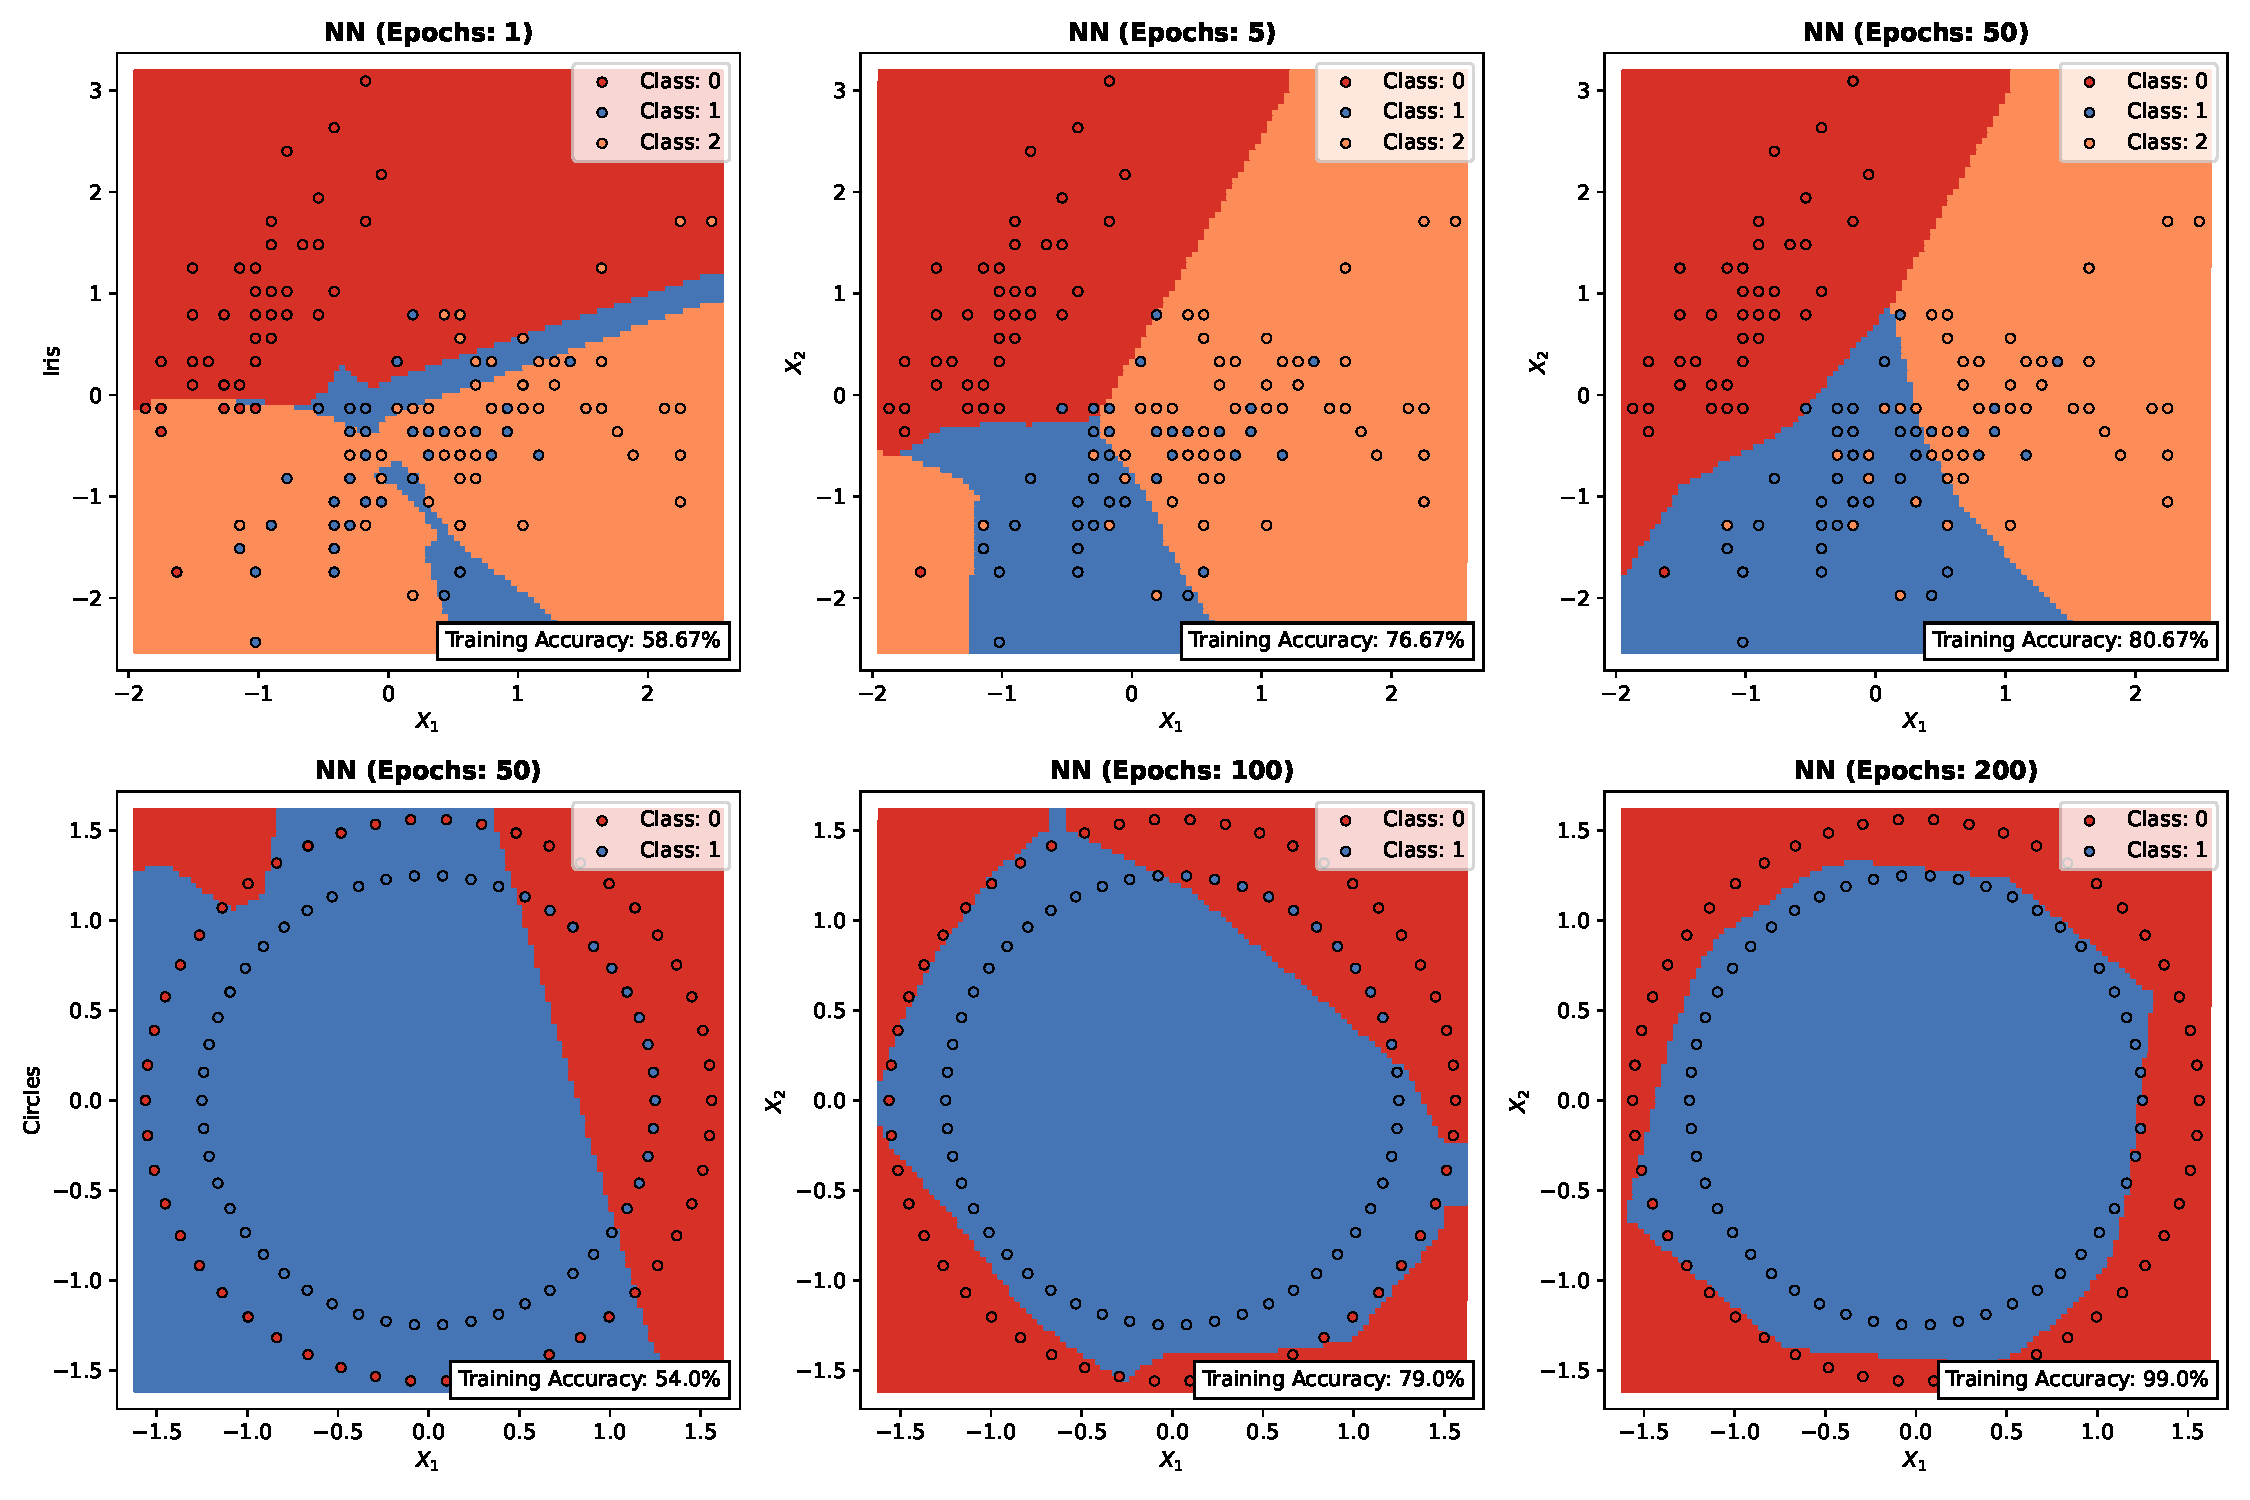
\includegraphics[scale=0.37]{figures/assert_nn_toydata.pdf}
\captionsetup{justification=centering,margin=2cm}
\caption{Performance of Neural Network on Iris (Row 1) and Circles (Row 2)}
\label{assert_nn_toydata}
\end{figure}